\documentclass{beamer}
\usetheme{Madrid}

\usepackage{amsmath, amssymb, amsthm}
\usepackage{graphicx}
\usepackage{listings}
\usepackage{gensymb}
\usepackage{minted}
\usemintedstyle{friendly}
\definecolor{bg}{rgb}{0.95,0.95,0.95}
\usepackage[utf8]{inputenc}
\usepackage{hyperref}
\usepackage{gvv}\begin{document}
\title{NCERT - 8.3.17}
\author{EE24BTECH11044 - MUTHYALA KOUSHIK$^{*}$}
\date{}
\frame{\titlepage}

\begin{frame}
\frametitle{Question}
The area bounded by the curve $y=x\abs{x}$, x-axis and the ordinates $x=-1$ and $x=1$ is given by 
\end{frame}

\begin{frame}{allowframebreaks}
\frametitle{Solution}
\begin{itemize}
  \item The function \( y = x |x| \) is piecewise defined:
  \[
  y = 
  \begin{cases} 
  x^2 & \text{if } x \geq 0, \\
  -x^2 & \text{if } x < 0.
  \end{cases}
  \]
  \item The area is computed as:
  \[
  A = \int_{-1}^{1} |y| \, dx.
  \]
\end{itemize}
\end{frame}

\begin{frame}
\frametitle{Splitting the Integral}
\begin{itemize}
  \item The function changes at \( x = 0 \), so split the integral:
  \[
  A = \int_{-1}^{0} \abs{-x^2} \, dx + \int_{0}^{1} x^2 \, dx.
  \]
  \item We evaluate each part separately.
\end{itemize}
\end{frame}

\begin{frame}
\frametitle{Evaluating the Integrals}
\begin{itemize}
  \item For the first integral:
  \[
  A_1 = \int_{-1}^{0} \abs{-x^2} \, dx =  \left[ \frac{x^3}{3} \right]_{-1}^{0} = \frac{1}{3}.
  \]
  \item For the second integral:
  \[
  A_2 = \int_{0}^{1} x^2 \, dx = \left[ \frac{x^3}{3} \right]_{0}^{1} = \frac{1}{3}.
  \]
  \item The total area is:
  \[
  A = A_1 + A_2 = \frac{1}{3} + \frac{1}{3} = \frac{2}{3}.
  \]
 Therefore, the area is:
\[
A = 0.66666666667.
\] 
\end{itemize}
\end{frame}

\begin{frame}{Numerical Solution Using Trapezoidal Rule}
\textbf{Numerical Solution:}
We can approximate the integral using the trapezoidal rule:
\[
J = \int_a^b f(x) \, dx \approx h \left( \frac{1}{2} f(a) + f(x_1) + f(x_2) + \cdots + f(x_{n-1}) + \frac{1}{2} f(b) \right),
\]
where \( h = \frac{b - a}{n} \) is the step size.

For our problem:
\[
A = A_n, \text{ where } A_{i+1} = A_i + h \cdot \frac{f(x_{n+1}) + f(x_n)}{2}.
\]
\[
A_{i+1} = A_i + \frac{h}{2} \left( f(x_{n+1}) + f(x_n) \right).
\]
\end{frame}

\begin{frame}{Numerical Solution}
\textbf{Iteration Formula:}
  \begin{itemize}
    \item \begin{align*}
      A_{i+1} &= A_i + \frac{h}{2} \left( {x_{n+1}}^2 + {x_n}^2 \right), \quad x_{n+1} = x_n + h.
    \end{align*}
  \end{itemize}
  The step size \( h = \frac{2}{n} \), where \( n \) is the number of subintervals. For this example, assume \( n = 1000 \). The initial conditions are:
\begin{itemize}
    \item \( a = -1 \),
    \item \( b = 1 \),
    \item \( A_0 = 0 \),
    \item \( h = \frac{2}{n} \).
\end{itemize}
We compute \( A \) iteratively until we reach the final area.
\end{frame}

\begin{frame}{Theoretical vs Computational Results}
The theoretical value of the area is:
\[
A = \frac{2}{3} \approx 0.66666666667.
\]
Using the trapezoidal rule, the computed value of the area is:
\[
A \approx 0.6666679999999998.
\]
Thus, the computed value is very close to the theoretical value, showing that the trapezoidal rule provides a good approximation.
\end{frame}

\begin{frame}
\frametitle{Plot}
\begin{figure}[h]
	\centering
	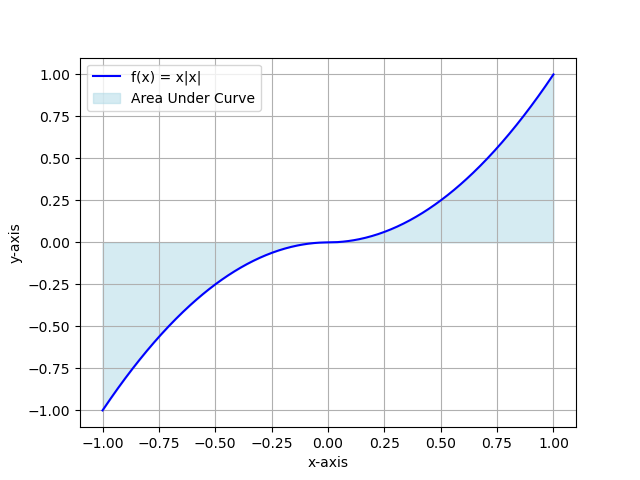
\includegraphics[scale=0.5]{figs/fig.png}
\end{figure}
\end{frame}

\end{document}
